\section{Design decisions}

\subsection{Database}
We use MongoDB for our database. We chose to use this database as it is easy to implement and easy to use. We have
a MongoDB database with 1 collection, Bikes. The Bikes collection stores all bike locations and their availability. There should be a second database collection, Users, for storing the name, passwords and a list of rented bikes. Due to lack of time, we weren't able to implement this correctly.


    \begin{figure}[H]
		\centering
		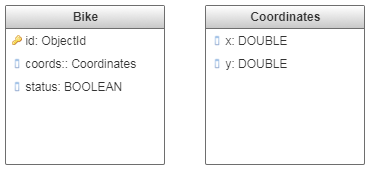
\includegraphics[width=0.4\textwidth]{images/db-structure.png}
		\caption{Overview of the database}
		\label{database}
	\end{figure}


\subsection{Webserver}
We chose Play as the framework for back-end development of our application mostly because it supports asynchronous I/O. There were two main causes for choosing Scala: the first is the possibility to learn a new programming language and the second is professor's incentive to use Scala for back-end development. In the end we succeeded in building a working back-end. We benefited from online completed projects we found on the internet as it aided our understanding and development of the final product. During the development we had difficulties connecting our database with Play as well as using WebSockets for live data streaming.

\subsection{Client}
Angular is a framework for building Web single-page applications and Bootstrap is an easy to use front-end web framework for designing web applications. These are the main reasons why we chose to use these frameworks. Other advantage of using Angular is its highly readable and comprehensive code. It was an important factor because we wanted something that will take as little time to learn as possible. We created the project using Angular Cli and used components to create the navigation bar, map component, and two (login and registration) forms (unfortunately not seen in the final layout). Even if it is not linked to framework itself, we found useful the large community of developers using Angular as online answers helped us solve most encountered problems.

\begin{figure}[H]
		\centering
		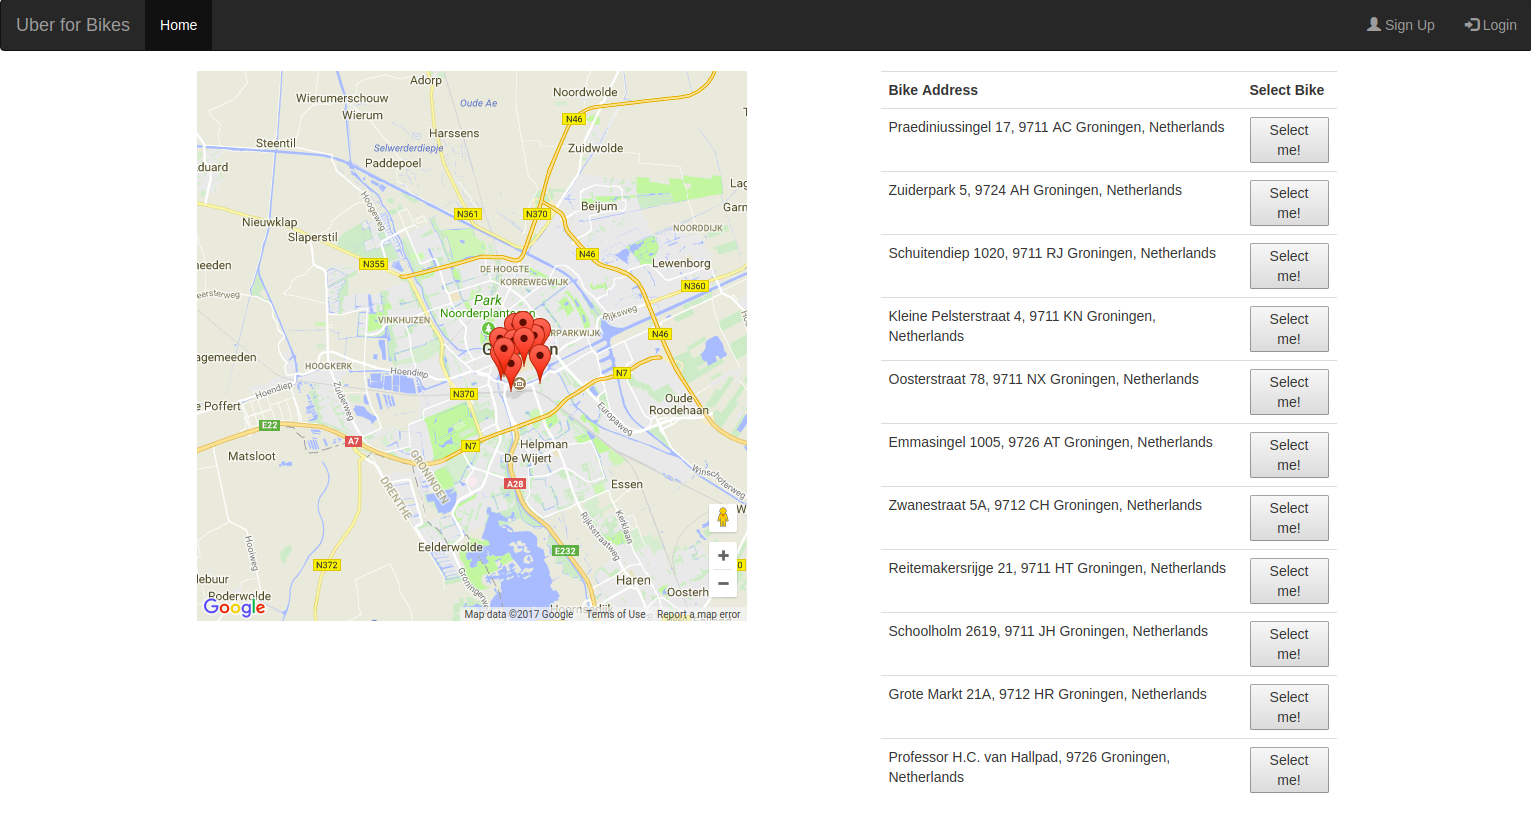
\includegraphics[width=0.9\textwidth]{images/screenshot.png}
		\caption{Application layout}
		\label{front-end}
	\end{figure}
